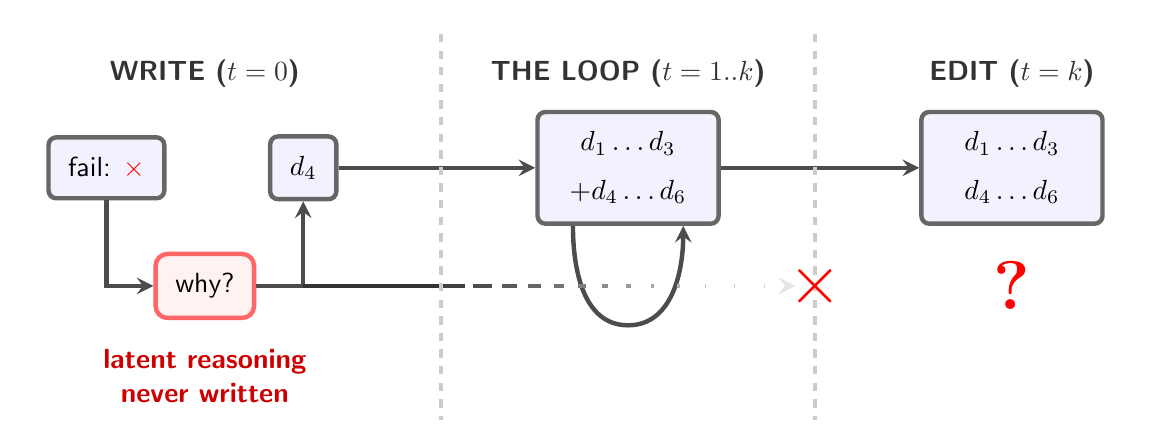
\begin{tikzpicture}[
    >=stealth,
    font=\sffamily,
    % Core styles: uniform standard font size, 1.6pt line widths (100% thicker)
    stage_title/.style={font=\sffamily\bfseries, text=black!80},
    mem/.style={draw=black!60, line width=1.6pt, rounded corners=1mm, fill=blue!5, align=center, inner sep=2.5mm},
    % why box explicitly defines the 2.5mm intra-box margin
    why/.style={draw=red!60, line width=1.6pt, rounded corners=1.5mm, fill=red!5, align=center, inner sep=2.5mm},
    ann/.style={font=\sffamily\bfseries, text=red!80!black, align=center},
    flow/.style={->, line width=1.6pt, draw=black!70}
  ]

  % Bounding box mathematically locked to 2.81 aspect ratio to prevent distortion (14 / 4.98)
  % Y=0.0 is precisely calibrated to match the header/box margin
  \useasboundingbox (0, 0) rectangle (14, 4.98);

  % ---------------------------------------------------------
  % PLANE 1: TEXT / TITLES (Y = 4.4)
  % ---------------------------------------------------------
  \node[stage_title] at (2.25, 4.4) {WRITE ($t=0$)};
  \node[stage_title] at (7.625, 4.4) {THE LOOP ($t=1..k$)};
  \node[stage_title] at (12.5, 4.4) {EDIT ($t=k$)};

  % ---------------------------------------------------------
  % PLANE 2: OBSERVABLES (Y = 3.2)
  % ---------------------------------------------------------
  \node[mem] (fail) at (1.0, 3.2) {fail: \textcolor{red}{\bfseries $\times$}};
  \node[mem] (d4) at (3.5, 3.2) {$d_4$};
  \node[mem, text width=1.8cm] (loopm) at (7.625, 3.2) {$d_1 \dots d_3$ \\ \vspace{2mm} $+d_4 \dots d_6$};
  \node[mem, text width=1.8cm] (readm) at (12.5, 3.2) {$d_1 \dots d_3$ \\ \vspace{2mm} $d_4 \dots d_6$};

  % Observable execution flows
  \draw[flow] (d4) -- (loopm);
  \draw[flow] (loopm) -- (readm);

  % ---------------------------------------------------------
  % PLANE 3: HIDDEN REASONING (Y = 1.7)
  % ---------------------------------------------------------
  \node[why] (why) at (2.25, 1.7) {why?};

  % Caption margin mathematically locked to exactly match the 2.5mm intra-box margin above
  \node[ann, anchor=north] at ([yshift=-2.5mm]why.south) {latent reasoning \\ never written};

  % Right-angled causal pathways
  \draw[flow] (fail.south) |- (why.west);
  \draw[flow] (why.east) -| (d4.south);

  % Depictive execution loop reaching deep into the reasoning plane (down to Y=1.2)
  \draw[flow] ([xshift=-0.7cm]loopm.south)
  to[out=270, in=180] (7.625, 1.2)
  to[out=0, in=270] ([xshift=0.7cm]loopm.south);

  % ---------------------------------------------------------
  % SMOOTH MANUAL DEGRADATION (X = 3.5 to X = 9.75)
  % ---------------------------------------------------------
  % Originates at the right-angle corner of the why->d4 arrow
  \draw[line width=1.6pt, draw=black!80] (3.5, 1.7) -- (5.25, 1.7); % Solid up to Write/Loop boundary

  % Exponentially decaying segment length, increasing gaps, and fading opacity
  \draw[line width=1.6pt, draw=black!75] (5.25, 1.7) -- (5.55, 1.7);
  \draw[line width=1.6pt, draw=black!70] (5.65, 1.7) -- (5.90, 1.7);
  \draw[line width=1.6pt, draw=black!65] (6.02, 1.7) -- (6.22, 1.7);
  \draw[line width=1.6pt, draw=black!60] (6.36, 1.7) -- (6.52, 1.7);
  \draw[line width=1.6pt, draw=black!55] (6.68, 1.7) -- (6.81, 1.7);
  \draw[line width=1.6pt, draw=black!50] (6.99, 1.7) -- (7.09, 1.7);
  \draw[line width=1.6pt, draw=black!45] (7.29, 1.7) -- (7.37, 1.7);
  \draw[line width=1.6pt, draw=black!40] (7.60, 1.7) -- (7.66, 1.7);
  \draw[line width=1.6pt, draw=black!35] (7.92, 1.7) -- (7.96, 1.7);
  \draw[line width=1.6pt, draw=black!30] (8.25, 1.7) -- (8.28, 1.7);
  \draw[line width=1.6pt, draw=black!25] (8.60, 1.7) -- (8.62, 1.7);
  \draw[line width=1.6pt, draw=black!20] (8.97, 1.7) -- (8.98, 1.7);
  \draw[line width=1.6pt, draw=black!15] (9.35, 1.7) -- (9.36, 1.7);
  \draw[->, line width=1.6pt, draw=black!10] (9.70, 1.7) -- (9.75, 1.7);

  % ---------------------------------------------------------
  % VERTICAL DIVIDERS AND BOUNDARY MARKERS
  % ---------------------------------------------------------
  \draw[dashed, black!20, line width=1.6pt] (5.25, 4.9) -- (5.25, 0.0);
  \draw[dashed, black!20, line width=1.6pt] (10.0, 4.9) -- (10.0, 0.0);

  % Degradation failure point exactly at the boundary (X=10.0)
  \node[text=red, font=\Huge\bfseries, inner sep=0pt] at (10.0, 1.7) {$\times$};

  % Read-time reasoning void
  \node[text=red, font=\Huge\bfseries] at (12.5, 1.7) {?};

\end{tikzpicture}
